\documentclass[tikz,border=10pt]{standalone}
\usepackage{tikz}
\usetikzlibrary{positioning}
\usetikzlibrary {arrows.meta}
\usetikzlibrary{calc}
\usepackage{unicode-math}
\setmathfont{XITS Math}
\begin{document}

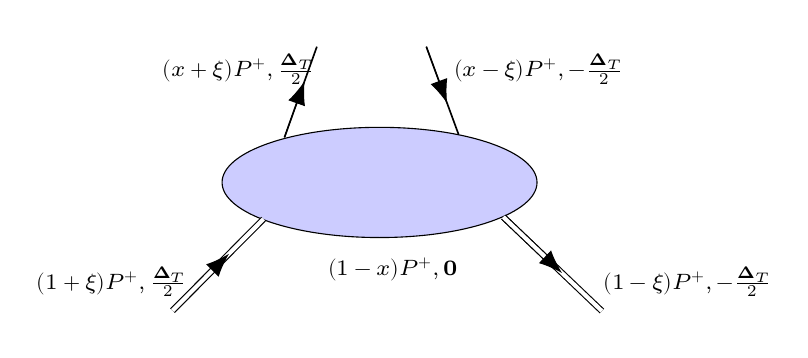
\begin{tikzpicture}[font=\footnotesize]
    \node (a0) at (0,0){};
    \node[above right =-.59   and -1.6 of a0] (a1){};
    \node[above right =-2   and -3 of a0] (b1){};
    \node[above right =-1.7   and -4.6 of a0] (b1l){$(1+\xi)P^+,\frac{\symbf\Delta_T}{2}$};
    \node[above right =-.57   and 1.2 of a0] (a2){};
    \node[above right =-2   and 2.7 of a0] (b2){};
    \node[above right =-1.7   and 2.6 of a0] (b2l){$(1-\xi)P^+,-\frac{\symbf\Delta_T}{2}$};
    \node[above right =.24   and .8 of a0] (a3){};
    \node[above right =1.6   and .3 of a0] (b3){};
    \node[above right =1   and .7 of a0] (b3l){$(x-\xi)P^+,-\frac{\symbf\Delta_T}{2}$};
    \node[above right =.2   and -1.5 of a0] (a4){};
    \node[above right =1.6   and -1 of a0] (b4){};
    \node[above right =1   and -3 of a0] (b4l){$(x+\xi)P^+,\frac{\symbf\Delta_T}{2}$};
    % 画椭圆
    \filldraw[fill=blue!20,draw=black] (a0) ellipse [x radius=2cm,y radius=.7cm];
    \node[above right =-1.5  and -.9 of a0] (b4l){$(1-x)P^+,\symbf 0$};
    %入射和出射部分子
    \draw[semithick] (b3)--(a3);
    \draw[-{Latex[length=3mm]} ] (b3)--($(b3)!.62!(a3)$);
    \draw[semithick] (b4)--(a4);
    \draw[-{Latex[length=3mm]} ] (a4)--($(a4)!.6!(b4)$);
    % 入射和出射核子
    \draw[double,double distance=1.5pt] (b1)--(a1);
    \draw[double,double distance=1.5pt,-{Latex[length=3mm]} ] (b1)--($(b1)!.6!(a1)$);
    \draw[double,double distance=1.5pt] (b2)--(a2);
    \draw[double,double distance=1.5pt,-{Latex[length=3mm]} ] (a2)--($(a2)!.58!(b2)$);
\end{tikzpicture}

\end{document}